%!TEX program = xelatex

\documentclass{progbookcn}
\usepackage{wrapfig}
\usepackage{enumerate}
\usepackage{amsmath,mathrsfs,amsfonts}
\usepackage{tabularx}
\usepackage{booktabs}
\usepackage{colortbl}
\usepackage{multirow,makecell}
\usepackage{multicol}
\usepackage{ulem} % \uline
\usepackage{listings}
\usepackage{tikz}
\usepackage{tcolorbox}
\usepackage{fontawesome}
\usepackage[open,openlevel=0,atend]{bookmark}
\usepackage{graphicx}
\usepackage{float}
\usepackage{imakeidx}
\usepackage{wrapfig}
\makeindex[%
  intoc=true,
  columns=2,
  columnsep=1cm,
  columnseprule=true
]


\begin{document}

%% title page
\begin{titlepage}
  \vspace*{25ex}

  \hspace{0.05\textwidth}\begin{minipage}{.9\textwidth}
    \flushright

    %%中文书名
    {\zihao{1}\textbf{在浏览器中设计, 训练, 测试神经网络}}

    \rule{\linewidth}{.5pt}

    \vspace{2ex}

    %% 英文书名
    {\zihao{3}\textsf{Designing, Training and Testing Neural Networks in Browser}} \\

    \vspace{20ex}

    %% 作者
    {\zihao{4}\textit{南京大学计算机科学与技术系Dislab}}\\
    {\zihao{4}\textit{马浩杰~~林明凯~~李文中}}\\
    {\zihao{4}\textit{中国·江苏省南京市栖霞区南京大学仙林校区}}\\
  \end{minipage}

  \vfill

  \centering
  {\zihao{4}南京 ~$\bullet$ ~NANJING}
\end{titlepage}
\thispagestyle{empty}


\frontmatter


%% 目录
\clearpage
{
  \hypersetup{hidelinks}
  \tableofcontents
}


\mainmatter

\part{VisualNN界面介绍}


\chapter{主体界面}

VisualNN是用于可视化建模神经网络的工具, 并提供模型导入导出, 在线训练的功能, 整个网站的界面如下所示

\begin{figure}[H]
  \centering
  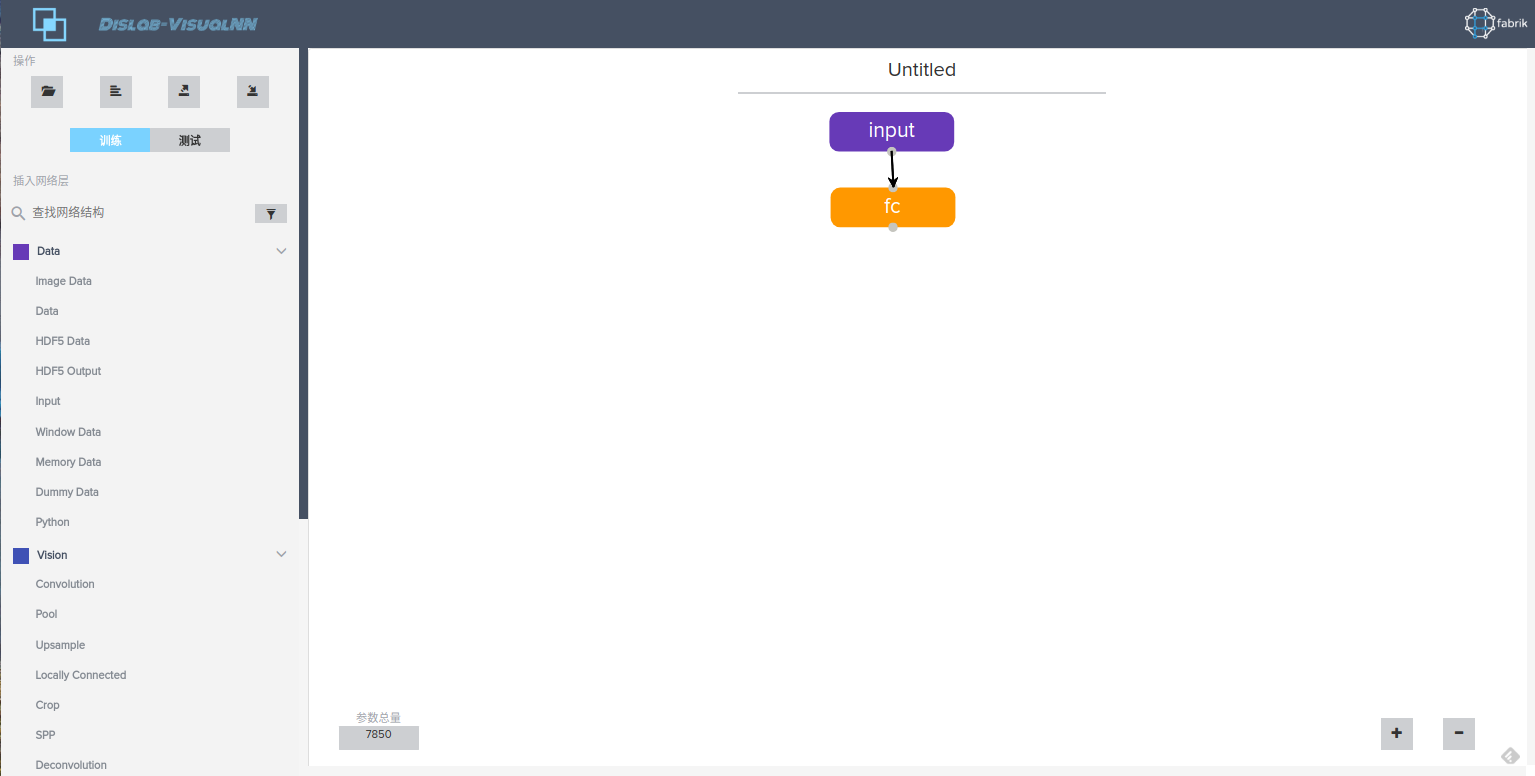
\includegraphics[width=0.98\linewidth]{screenshot.png}
\end{figure}

主要组成有三个部分, 左侧是神经网络单元工具箱, 中间是神经网络架构图, 右侧是网络单元参数设置界面, 可以通过拖拉拽左侧的网络单元到中间来自行搭建神经网络模型, 也可以导入系统提供的很多经典模型. 下面分节讲述每个部分的使用方法.



\section{工具栏介绍}

具体的工具栏如下图所示, 从左到右分别提供了model zoo, load from text, export, import的功能.

\begin{figure}[H]
  \centering
  
\includegraphics{toolbar.png}
\end{figure}


\subsection{model zoo}

model zoo使得用户能够直接导入一些已经设计好的经典模型, 具体界面如下所示, 目前系统还处于原型阶段, 尚未提供网络结构.
\begin{figure}[H]
  \centering
  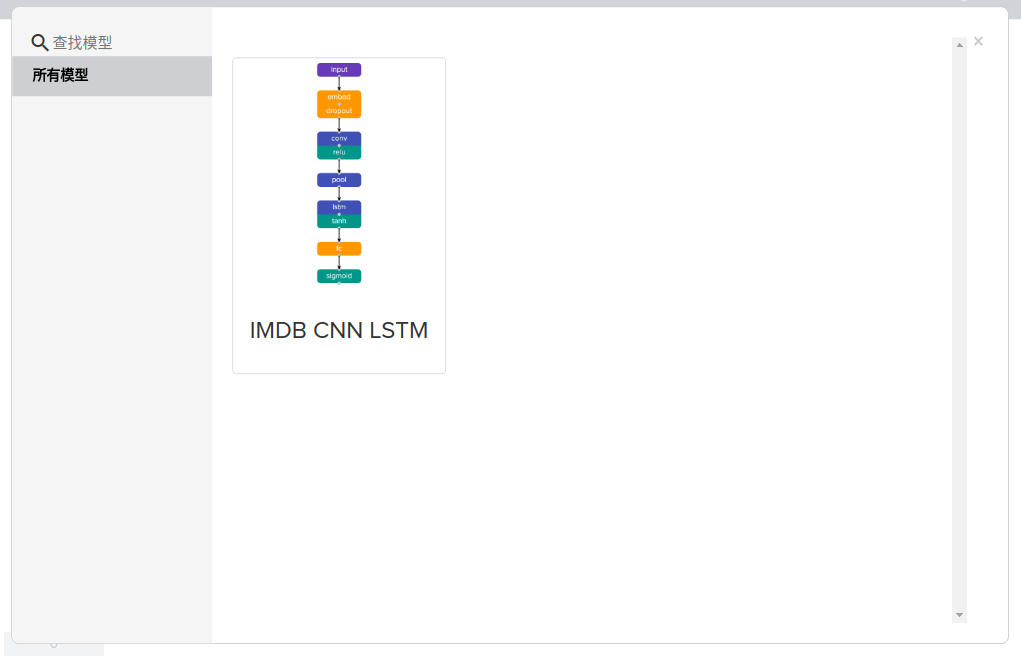
\includegraphics[width=0.98\linewidth]{model_zoo.png}
\end{figure}


\subsection{load from text}

这项功能使得用户可以通过json格式或者pb格式的输入直接导入网络结构, 具体界面如下所示:
\begin{figure}[H]
  \centering
  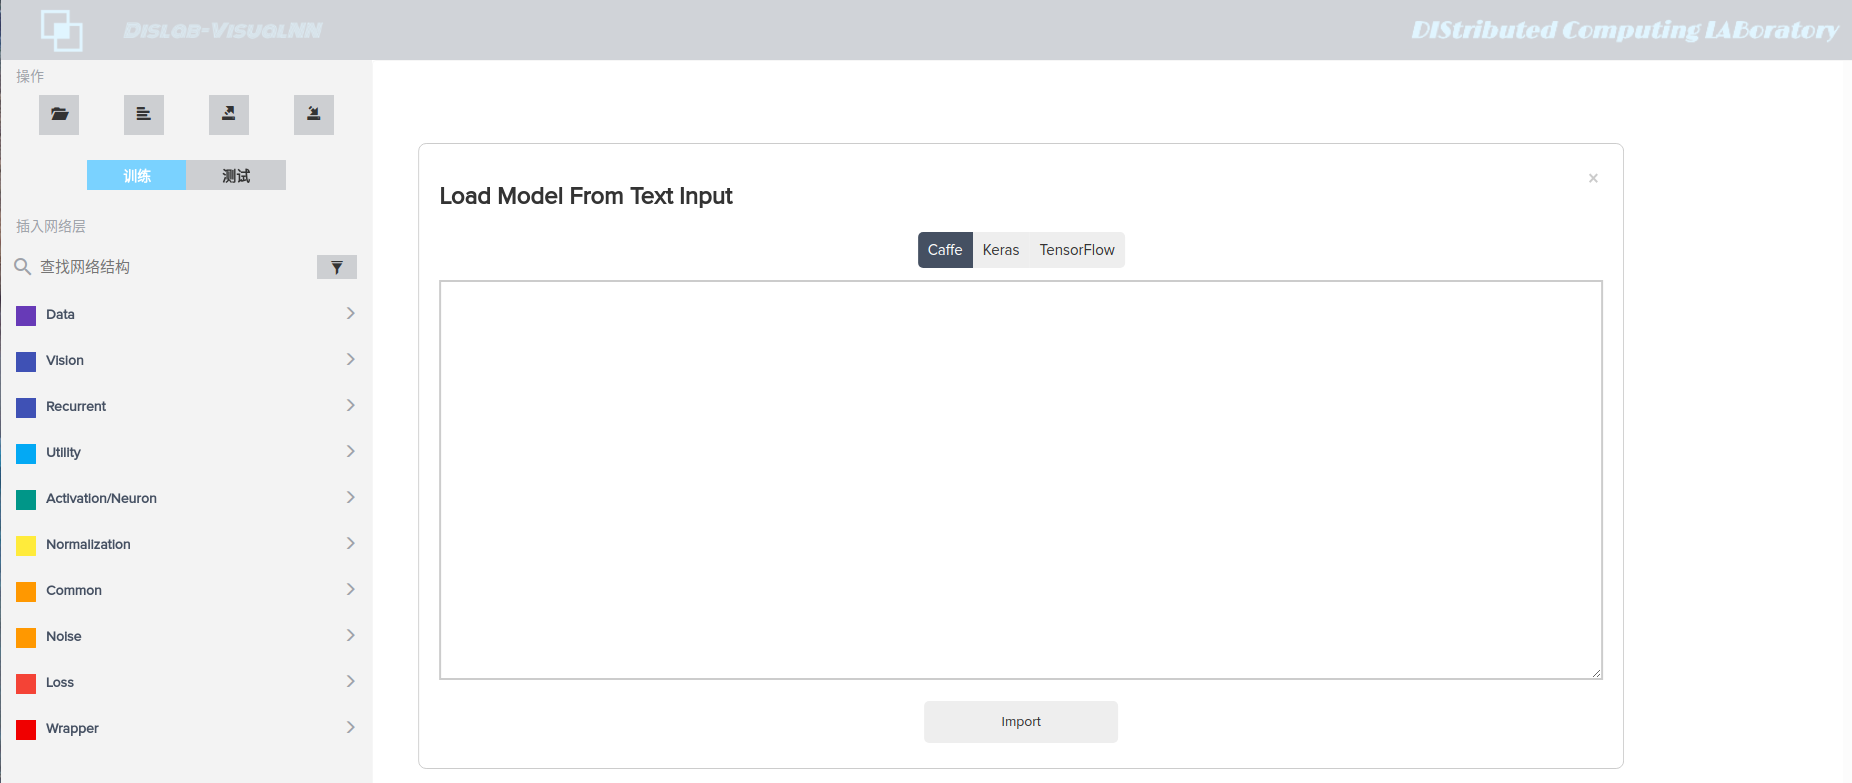
\includegraphics[width=0.98\linewidth]{load_from_text.png}
\end{figure}

\subsection{export功能}

用户可以通过export按钮从磁盘导入json或者pbtxt格式的模型文件, 如下图
\begin{figure}[H]
  \centering
  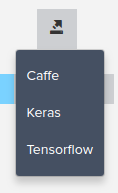
\includegraphics{export.png}
\end{figure}

\subsection{import功能}

用户可以通过import按钮将网页中设计好的神经网络文件导出为json或者pbtxt格式的文件输出到磁盘上, 如下图所示
\begin{figure}[H]
  \centering
  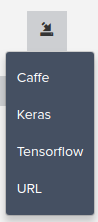
\includegraphics{import.png}
\end{figure}

\section{神经网络组件}

VisualNN提供一些基本的网络单元来进行神经网络设计, 具体界面如下

\begin{figure}[H]
  \centering
  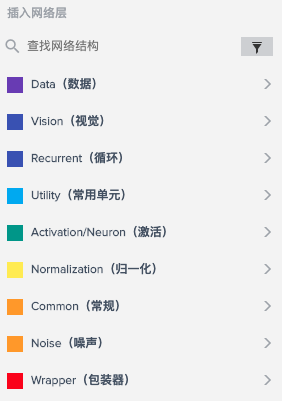
\includegraphics[scale = 0.6]{network_unit.png}
\end{figure}

从上到下分别由Data(数据层), Vision(视觉层), Recurrent(循环层), Utility(常用单元层), Activation(激活层), Normalization(归一化层), Common(常规层), Noise(噪声层),  Wrapper(包装器层)构成. 通过选择组件中的常用组件可以自行绘制出一张神经网络图用于训练。同时可以调整神经网络中的参数。

\begin{figure}[H]
  \centering
  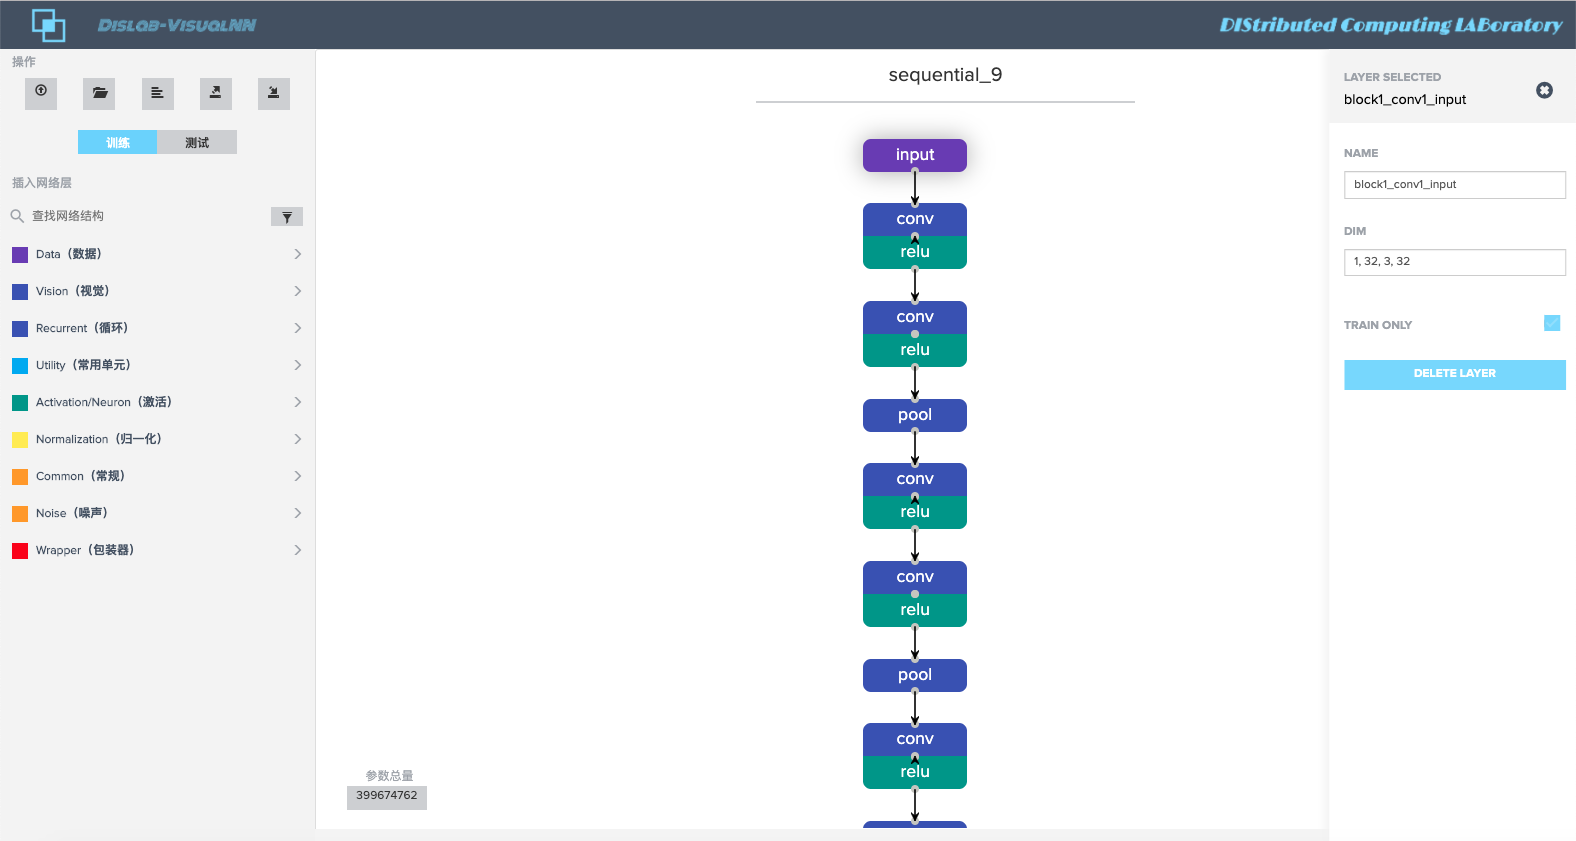
\includegraphics[width=0.98\linewidth]{draw.png}
\end{figure}






\chapter{神经网络组件}

神经网络组件对应于构造神经网络基本组成部分,主要由九个部分组成,分别是Data(数据层), Vision(视觉层), Recurrent(循环层), Utility(常用单元层), Activation(激活层), Normalization(归一化层), Common(常规层), Noise(噪声层),  Wrapper(包装器层)通过这些部分中的下属组件,就可以利用可视化的拖拽方式构造神经网络模型,这里主要介绍组件及其作用。

\section{数据层(Data)}

data\_layer应该是⽹网络的最底层,主要是将数据送给blob进⼊入到net中,在data\_layer中仅有⼀一个input 标签,⽤用于设置数据的输入,可以在属性中设置数据的输入形状(Keras,Tensorflow)。

\begin{figure}[H]
  \centering
  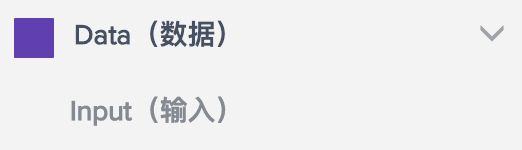
\includegraphics[scale = 0.6]{Data_layer.png}
\end{figure}




\section{视觉层(vision)}

视觉层通常将图像作为输入并产生其他图像作为输出,尽管它们可以获取其他类型和尺寸的数据。现实世界中的典型“图像”可以具有一个颜色通道(channel
= 1),如灰度图像,或三个颜色通道(channel = 3),如RGB(红色,绿色,蓝色) 图片。特别地,大多数视觉层通过将特定操作应用于输入的某个区域来工作以产生输出的相应区域。其中包括六个部分,分别是卷积层(Convolution)、池化层(Pool)、升采样(Upsample)、局部连接层(Locally Connected)、Deconvolution(反卷积)、Depthwise Convolution(深度卷积)。
\begin{figure}[H]
  \centering
  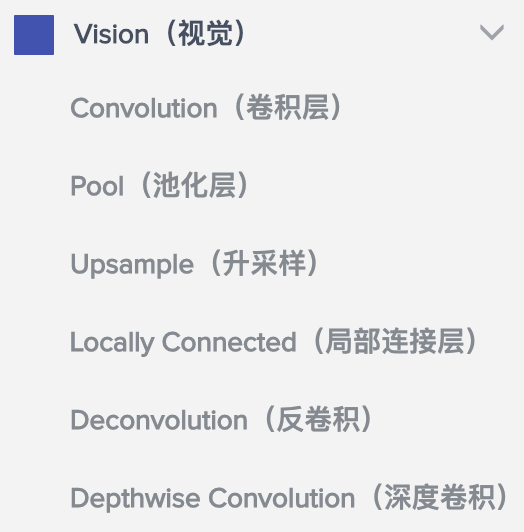
\includegraphics[scale = 0.6]{Vision_layer.png}
\end{figure}

\begin{itemize}
\item 卷积层(Convolution)(Keras,Tensorflow)

  ​	卷积神经网络(CNN)第一次提出是在1997年,杨乐春(LeNet)的一篇关于数字OCR识别的论文,在2012年的ImageNet竞赛中CNN网络成功击败其它非DNN模型算法,从此获得学术界的关注与工业界的兴趣。卷积神经网络中每层卷积层(Convolutional layer)由若干卷积单元组成,每个卷积单元的参数都是通过反向传播算法最佳化得到的。卷积运算的目的是提取输入的不同特征,第一层卷积层可能只能提取一些低级的特征如边缘、线条和角等层级,更多层的网路能从低级特征中迭代提取更复杂的特征。在VisualNN系统中可以通过卷积层来设置1D,2D,3D等参数来设置不同类型的卷积层。

\item 池化层(Pool)(Keras,Tensorflow)

  ​	在CNN网络中卷积池之后会跟上一个池化层也叫下采样层,池化层的作用是提取局部均值与最大值,根据计算出来的值不一样就分为均值池化层与最大值池化层,一般常见的多为最大值池化层。池化层可以非常有效地缩小参数矩阵的尺寸,从而减少最后全连层中的参数数量。使用池化层即可以加快计算速度也有防止过拟合的作用。池化的时候同样需要提供filter的大小、步长等参数。池化还能降低输出结果的维度,(理想情况下)却能保留显著的特征。

\item 升采样(Upsample)(Keras)

  ​	升采样,也即插值。对于图像来说即是二维插值,图像放大几乎都是采用内插值方法,即在原有图像像素的基础上在像素点之间采用合适的插值算法插入新的元素。如果升采样系数为$k$,即在原图$n$与$n+1$两点之间插入$k-1$个点,使其构成$k$分。二维插值即在每行插完之后对于每列也进行插值。 插值的方法分为很多种,一般主要从时域和频域两个角度考虑。对于时域插值,最为简单的是线性插值。除此之外,Hermite插值,样条插值等等均可以从有关数值分析书中找到公式,直接代入运算即可。对于频域,根据傅里叶变换性质可知,在频域补零等价于时域插值。所以,可以通过在频域补零的多少实现插值运算。在VisualNN系统中可以通过升采样层来设置1D,2D,3D等参数来设置不同类型的升采样层。

\item 局部连接层(Locally Connected)(Keras)

  ​	局部连接网络。每个隐含单元仅仅连接输入图像的一小片相邻区域,那么这就是一种局部连接方式。网络部分连通的思想,是受启发于生物学里面的视觉系统结构,视觉皮层的神经元就是局部接受信息的(即这些神经元只响应某些特定区域的刺激)。利用这样一种局部连接结构,一方面降低了需要学习的参数数量,提高了前向传播和反向传播的计算速度;另一方面,这种结构所具有的局部感受能力也更符合人类视觉系统的认知方式。同时,卷积神经网络真正实现了端到端的学习,一个网络结构包括了特征提取和分类两部分,更适合实际业务中的算法部署。在VisualNN系统中可以通过升采样层来设置1D、2D等参数来设置不同类型的局部连接层。

\item 反卷积层(Deconvolution)(Keras,Tensorflow)

  ​	反卷积(Deconvolution)的概念第一次出现是Zeiler在2010年发表的论文Deconvolutional networks中,但是并没有指定反卷积这个名字,反卷积这个术语正式的使用是在其之后的工作中。随着反卷积在神经网络可视化上的成功应用,其被越来越多的工作所采纳比如:场景分割、生成模型等。其中反卷积(Deconvolution)也有很多其他的叫法,比如:Transposed Convolution,Fractional Strided Convolution等等。卷积计算对应的反卷积操作的输入输出关系正好相反,卷积层输入多个,输出单一的激活值,反卷积输入一个,输出多个激活值。如果不考虑通道以卷积运算的反向运算来计算反卷积运算的话,我们还可以通过离散卷积的方法来求反卷积。 

\item 深度卷积层(Depthwise Convolution)(Keras,Tensorflow)

  ​	深度卷积是对输入的每一个channel独立的用对应channel的所有卷积核去卷积,假设卷积核的shape是[filter\_height, filter\_width, in\_channels, channel\_multiplier],那么每个in\_channel会输出channel\_multiplier那么多个通道,最后的feature map就会有in\_channels * channel\_multiplier个通道了。反观普通的卷积,输出的feature map一般就只有channel\_multiplier个通道。在Keras与TensorFlow中都提供了深度卷积层的实现。

\end{itemize}




\section{循环层(Recurrent)}

循环层(Recurrent Layer)在Keras中是循环层的抽象类,一般不在在模型中直接应用该层(因为它是抽象类,无法实例化任何对象)。一般使用它的子类LSTM,GRU或SimpleRNN来实现,因此VsualNN也提供了三种不同类型的循环神经网络的标签以供使用。分别是RNN(循环神经网络)、GRU(门控循环单元)、LSTM(长短期记忆网络)。
\begin{figure}[H]
  \centering
  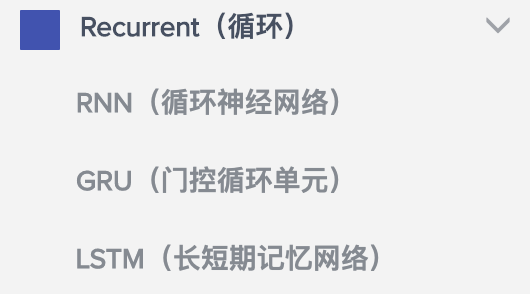
\includegraphics[scale = 0.6]{Recurrent_layer.png}
\end{figure}


\begin{itemize}
\item 循环神经网络(RNN)(Keras)

  ​	循环神经网络(Recurrent Neural Network,RNN)是一类专门用于处理时序数据样本的神经网络,它的每一层不仅输出给下一层,同时还输出一个隐状态,给当前层在处理下一个样本时使用。就像卷积神经网络可以很容易地扩展到具有很大宽度和高度的图像,而且一些卷积神经网络还可以处理不同尺寸的图像,循环神经网络可以扩展到更长的序列数据,而且大多数的循环神经网络可以处理序列长度不同的数据。它可以看作是带自循环反馈的全连接神经网络。循环神经网络的一个重要特性是:在不同时刻,模型的参数是共享的,这使得我们可以在时间上共享不同位置的统计强度。

\item 长短期记忆网络(LSTM)(Keras)

  ​	时序反向传播算法按照时间的逆序将错误信息一步步地往前传递。当每个时序训练数据的长度较大或者时刻较小时,损失函数关于时刻隐藏层变量的梯度比较容易出现消失或爆炸的问题(也称长期依赖问题)。梯度爆炸的问题一般可以通过梯度裁剪来解决,而梯度消失问题则要复杂的多,人们进行了很多尝试,其中一个比较有效的版本是长短期记忆神经网络(Long Short-Term Memory,LSTM)。LSTM 的主要思想是:门控单元以及线性连接的引入 。LSTM区别于RNN的地方,主要就在于它在算法中加入了一个判断信息有用与否的“处理器”,这个处理器作用的结构被称为cell。一个cell当中被放置了三扇门,分别叫做输入门、遗忘门和输出门。一个信息进入LSTM的网络当中,可以根据规则来判断是否有用。只有符合算法认证的信息才会留下,不符的信息则通过遗忘门被遗忘。LSTM可以在反复运算下解决神经网络中长期存在的大问题。目前已经证明,LSTM是解决长序依赖问题的有效技术,并且这种技术的普适性非常高,导致带来的可能性变化非常多。

\item 门控循环单元(GRU)(Keras)

  ​	GRU即Gated Recurrent Unit。前面说到为了克服RNN无法很好处理远距离依赖而提出了LSTM,而GRU则是LSTM的一个变体,当然LSTM还有有很多其他的变体。GRU保持了LSTM的效果同时又使结构更加简单,所以它也非常流行。而GRU模型只有两个门,分别为更新门和重置门。更新门用于控制前一时刻的状态信息被带入到当前状态中的程度,更新门的值越大说明前一时刻的状态信息带入越多。重置门用于控制忽略前一时刻的状态信息的程度,重置门的值越小说明忽略得越多。

\end{itemize}


\section{常用单元(Utility)}

常用单元(Utility)实用单元中集成了对于神经网络中网络层的一些实用的工具,用于规整,连接,切分向量等操作。在VisualNN系统中提供了九个工具操作,它们分别是扁平化(Flatten)、变形(Reshape)、连结(Concat)、Eltwisw、Softmax、Permute、重复向量(Repeat Vector)、正则化(Regularization)、遮蔽(Masking)。
\begin{figure}[H]
  \centering
  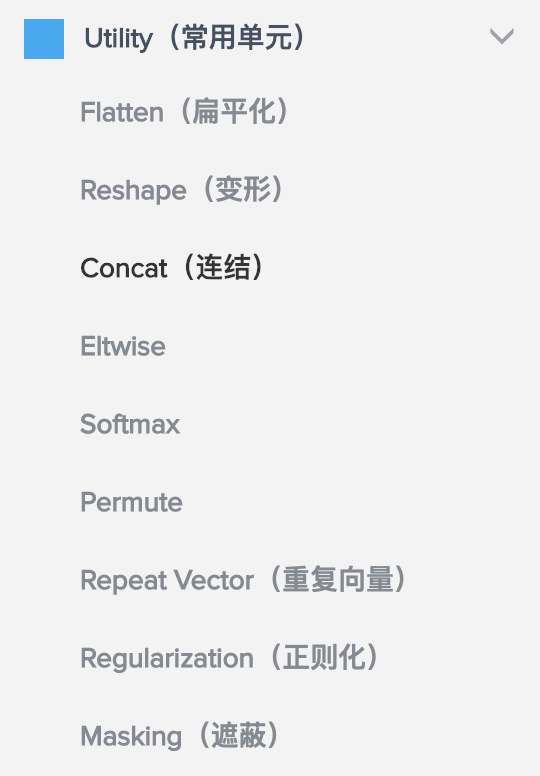
\includegraphics[scale = 0.6]{Utility_layer.png}
\end{figure}

\begin{itemize}
\item 扁平化(Flatten)(Keras,Tensorflow)

  ​	Flatten层用来将输入“压平”,即把多维的输入一维化,常用在从卷积层到全连接层的过渡。Flatten不影响batch的大小。

\item 变形(Reshape)(Keras)

  ​	Reshape层用来将输入shape转换为特定的shape

\item 连结(Concat)(Keras,Tensorflow)

  ​	其作用是将向量按照指定的维度进行连接。

\item Eltwise(Keras,Tensorflow)

  ​	针对于两个向量,Eltwise层的操作有三个:product(对应相乘), sum(相加减),max(取大值),Average(取平均),Dot(点乘),其中sum是默认操作。

\item Softmax(Keras,Tensorflow)

  ​	Softmax 函数可以把它的输入,通常被称为 logits 或者 logit scores,处理成 0 到 1 之间,并且能够把输出归一化到和为 1。

\item Permute(Keras)

  ​	Permute层将输入的维度按照给定模式进行重排,例如,当需要将RNN和CNN网络连接时,可能会用到该层。

\item 重复向量(Repeat Vector)(Keras)

  ​	Repeat Vector标签用于将输入输入向量重复n次。

\item 正则化(Regularization)(Keras)

  ​	数据量比较小会导致模型过拟合, 使得训练误差很小而测试误差特别大. 通过在Loss Function 后面加上正则项可以抑制过拟合的产生. 缺点是引入了一个需要手动调整的hyper-parameter。经过本层的数据不会有任何变化,但会基于其激活值更新损失函数值。VisualNN提供L1与L2两个正则化项。

\item 遮蔽(Masking)(Keras)

  ​	使用给定的值对输入的序列信号进行“屏蔽”,用以定位需要跳过的时间步。对于输入张量的时间步,即输入张量的第1维度(维度从0开始算),如果输入张量在该时间步上都等于mask value,则该时间步将在模型接下来的所有层(只要支持masking)被跳过(屏蔽)。

\end{itemize}



\section{激活层(Activation/Neuron)}

激活层(Activation/Neuron)激活函数也是神经网络中一个很重的部分。每一层的网络输出都要经过激活函数。VisualNN提供了比较常用了几个激活函数:ReLU/Leaky-ReLU、PReLU、ELU、Threshold ReLU、SELU、Softplus、Softsign、Sigmod、TanH、Hard Sigmod。
\begin{figure}[H]
  \centering
  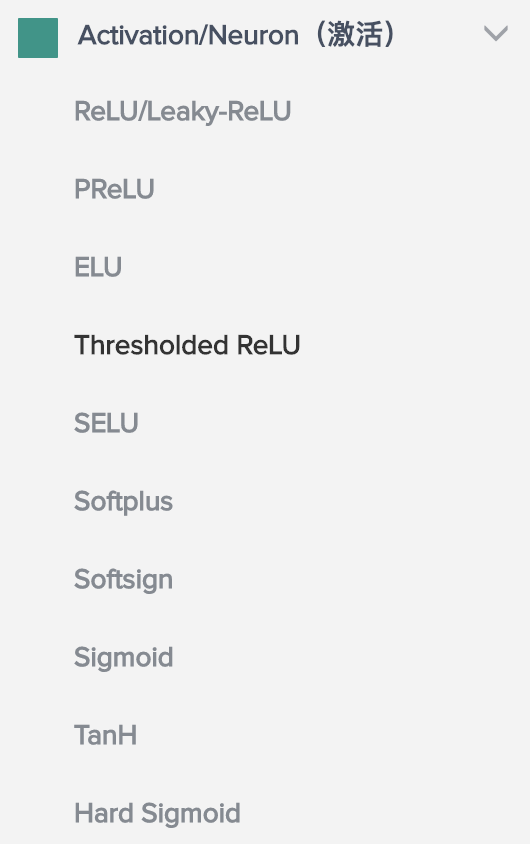
\includegraphics[scale = 0.6]{Activation_layer.png}
\end{figure}

\begin{itemize}
\item ReLU/Leaky-ReLU(Keras,Tensorflow)

  ​	ReLU是将所有的负值都设为零,相反,Leaky ReLU是给所有负值赋予一个非零斜率。Leaky ReLU激活函数是在声学模型(2013)中首次提出的。以数学的方式我们可以表示为:

  ​						 $y_i=\begin{cases}
  x_i (x_i\geq 0)\\
  \frac{x_i}{a_i} (x_i< 0)\\
  \end{cases}$

\item PReLU(Keras)

  ​	PReLU可以看作是Leaky ReLU的一个变体。在PReLU中,负值部分的斜率是根据数据来定的,而非预先定义的。在ImageNet分类(2015,Russakovsky等)上作者称,PReLU是超越人类分类水平的关键所在。

\item ELU(Keras,Tensorflow)

  ​	ELU函数曲线为:

  ​					$f(x)=\begin{cases}
  x (x\geq 0)\\
  \alpha(e^x-1) (x< 0)\\
  \end{cases}$

  该函数融合了sigmoid和ReLU,左侧具有软饱和性,右侧无饱和性。右侧线性部分使得ELU能够缓解梯度消失,而左侧软饱能够让ELU对输入变化或噪声更鲁棒。ELU的输出均值接近于零,所以收敛速度更快。

\item Threshold ReLU(Keras)

  该层是带有门限的ReLU,表达式是:

  ​						$f(x)=\begin{cases}
  x (x\geq \theta)\\
  0 (x<  \theta)\\
  \end{cases}$

\item SELU(Keras,Tensorflow)

  ​					$f(x)=\lambda\begin{cases}
  x (x\geq 0)\\
  \alpha(e^x-1) (x< 0)\\
  \end{cases}$

  ​	SELU为ELU乘上$\lambda$,该$\lambda$是大于1的。以前relu,prelu,elu这些激活函数,都是在负半轴坡度平缓,这样在activation的方差过大的时候可以让它减小,防止了梯度爆炸,但是正半轴坡度简单的设成了1。而selu的正半轴大于1,在方差过小的的时候可以让它增大,同时防止了梯度消失。这样激活函数就有一个不动点,网络深了以后每一层的输出都是均值为0方差为1。

\item Softplus(Keras,Tensorflow)

  ​	Softplus函数是Logistic-Sigmoid函数原函数,$f(x)=\log(e^x+1)$。由于$(1+e^x)$后期梯度过大,难以训练,于是增加log来减缓上升趋势。加1保证非负性。同年,Charles Dugas等人在NIPS会议论文中说明Softplus可以看作是强制非负校正函数$\max(0,x)$平滑版本。

\item Sigmod(Keras,Tensorflow)

  ​	Sigmoid$f(x)=\frac{1}{1+e^x}$函数是一个在生物学中常见的S型函数,也称为S型生长曲线。在信息科学中,由于其单增以及反函数单增等性质,Sigmoid函数常被用作神经网络的阈值函数,将变量映射到$(0,1)$之间。

\item TanH(Keras,Tensorflow)

  ​	TanH的函数为:$f(x)=\frac{e^x-e^{-x}}{e^x+e^{-x}}$,也称为双切正切函数,取值范围为$[-1,1]$。TanH在特征相差明显时的效果会很好,在循环过程中会不断扩大特征效果。与 sigmoid的区别是,TanH 是 0 均值的,因此实际应用中 TanH 会比 sigmoid 更好。

\item Hard Sigmod(Keras)

  ​	Hard Sigmod($f(x)=\max(0,\min(1,\frac{x+1}{2}))$是Logidtic Sigmod激活函数的分段近似。它更容易计算,这使得学习计算的速度更快,尽管首次派生值为0可能导致静默神经元/过慢的的学习速率。
\end{itemize}

\section{归一化层(Normalization)}

归一化层(Normalization)是能够对输入输出进行归一化操作的结构层,为Keras与Tensorflow所拥有的结构层,含有两个部分,分别是局部相应归一化(LRN)和批量归一化(Batch Norm)。
\begin{figure}[H]
  \centering
  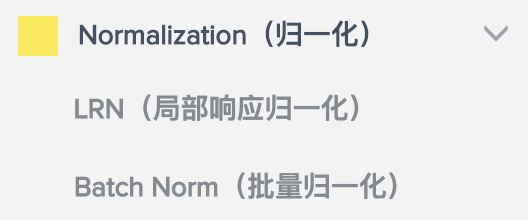
\includegraphics[scale = 0.6]{Normalization_layer.png}
\end{figure}

\begin{itemize}

\item 局部相应归一化(LRN)(Keras,Tensorflow)

  ​					$b^i_{x,y}=\frac{a^i_{x,y}}{k+\alpha \sum_{j=\max(0,i-\frac{n}{2})}^{{\min(N-1,i+\frac{n}{2})}}(a^i_{x,y})^2}$

  ​	局部归一的动机:在神经生物学有一个概念叫做侧抑制(lateral inhibitio),指的是被激活的神经元抑制相邻神经元。归一化(normalization)的目的是“抑制”,局部响应归一化就是借鉴侧抑制的思想来实现局部抑制,尤其当我们使ReLU的时候这种“侧抑制”很管用。LRN层模仿生物神经系统的侧抑制机制,对局部神经元的活动创建竞争机制,使得响应比较大的值相对更大,提高模型范化能力。在Hintonl的Imagenet中表明分别提升1.4\%和1.2\%,$a$表示第$i$个核在位置$(x,y)$运用ReLU非线性化神经元输出,$n$是同一位置上临近的kernel map的数目,$N$是也是kemel的总数。

\item 批量归一化(Batch Norm)(Keras,Tensorflow)

  ​	批量归一化对输入数据做了归一化处理,就是将每个特征在所有样本上的值转归一化成均值0方差1。这样我们保证训练数据里数值都同样量级上,从而使得训练的时候数值更加稳定。对于浅层模型来说,通常数据归一化预处理足够有效。输出数值在只经过几个神经层后通常不会出现剧烈变化。但对于深层神经网络来说,情况一般比较复杂。因为每一层里都对输入乘以权重后得到输出。当很多层这样的相乘累计在一起时,一个输出数据较大的改变都可以导致输出产生巨大变化,从而带来不稳定性。批量归一化层的提出是针对这个情况。它将一个批量里的输入数据进行归一化然后输出。如果我们将批量归一化层放置在网络的各个层之间,那么就可以不断的对中间输出进行调整,从而保证整个网络的中间输出的数值稳定性。

\end{itemize}


\section{ 常规层(Common)}

常规层(Common)是神经网络最为常规的一部分,主要包含了三个部分,分别是全连接层(Inner Product)、舍弃(Dropout)和嵌入(Embed)。
\begin{figure}[H]
  \centering
  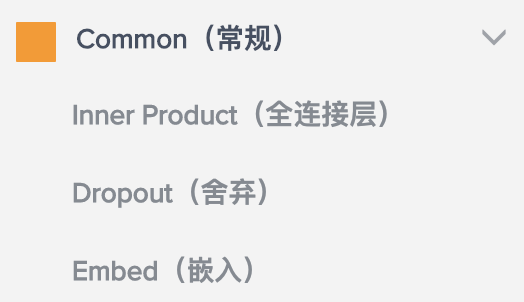
\includegraphics[scale = 0.6]{Common_layer.png}
\end{figure}

\begin{itemize}
\item 全连接层(Inner Product)(Keras,Tensorflow)

  ​	Inner Product即是全连接层,图像分类中,网络结构的最后一般有一个或多个全连接层。全连接层的每个节点都与其上层的所有节点相连,以综合前面网络层提取的特征。其全连接性,导致参数较多.全连接层将卷积的 2D 特征图结果转化为 1D 向量。

\item 舍弃(dropout)(Keras,Tensorflow)

  ​	Dropout可以作为训练深度神经网络的一种trick供选择。在每个训练批次中,通过忽略部分的特征检测器(让部分的隐层节点值为0),可以明显地减少过拟合现象。这种方式可以减少特征检测器(隐层节点)间的相互作用,检测器相互作用是指某些检测器依赖其他检测器才能发挥作用。Dropout说的简单一点就是:我们在前向传播的时候,让某个神经元的激活值以一定的概率$p$停止工作,这样可以使模型泛化性更强,因为它不会太依赖某些局部的特征

\item 嵌入(Embed)(Keras)

  ​	Embed层只能作为模型的第一层,是针对NLP的,将原始One-Hot编码的词(长度为词库大小)映射到低维向量表达,降低特征维数。
\end{itemize}


\section{ 噪声层(Noise)}

噪声层(Noise)在Keras中是的抽象类,主要是在输入数据中加入噪声,减轻过拟合的现象。VisualNN中提供了三种噪声方式:加性高斯噪声(Gaussian Noise)、乘性高斯噪声(Gaussian Dropout)、Alpha Dropout。
\begin{figure}[H]
  \centering
  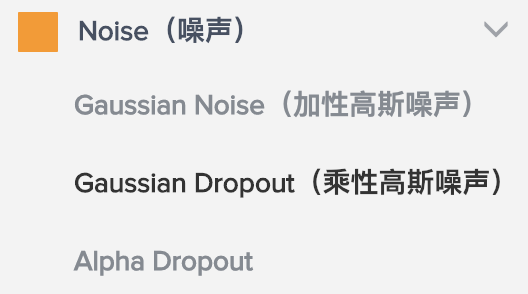
\includegraphics[scale = 0.6]{Noise_layer.png}
\end{figure}

\begin{itemize}
\item 加性高斯噪声(Gaussian Noise)(Keras)

  ​	为数据施加0均值,标准差为$\sigma$的加性高斯噪声。该层在克服过拟合时比较有用,你可以将它看作是随机的数据提升。高斯噪声是需要对输入数据进行破坏时的自然选择。因为这是一个起正则化作用的层,该层只在训练时才有效。

\item 乘性高斯噪声(Gaussian Dropout)(Keras)

  为层的输入施加以1为均值,标准差为$\sqrt{p/(1-p)}$的乘性高斯噪声。因为这是一个起正则化作用的层,因此该层只在训练时才有效。

\item Alpha Dropout(Keras)	

  ​	Alpha Dropout是一种保持输入均值和方差不变的Dropout,该层的作用是即使在dropout时也保持数据的自规范性。 通过随机对负的饱和值进行激活,Alphe Drpout与selu激活函数配合较好。
\end{itemize}


\section{  包装器层(Wrapper)}

包装器层(Wrapper)为Keras所特有,主要包括两个包装器,分别是时间分布包装器(Time Distributed)和双向RNN包装器(Bidirectional)。
\begin{figure}[H]
  \centering
  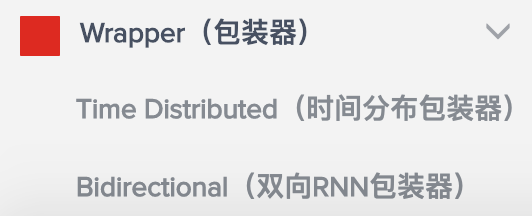
\includegraphics[scale = 0.6]{Wrapper_layer.png}
\end{figure}

\begin{itemize}
\item 时间分布包装器(Time Distributed)(Keras)	

  ​	输入至少为3D张量,下标为1的维度将被认为是时间维。在搭建需要独立连接时的结构时需要用到,比如在faster rcnn中,在最后fast rcnn的结构中进行类别判断和box框的回归时,需要对num\_rois个感兴趣区域ROIs进行回归处理,每一个区域的处理是相对独立的,等价于此时的时间步为num\_rois。

\item 双向RNN包装器(Bidirectional)(Keras)	

  ​	Bidirectional 是RNN的双向封装器,对序列进行前向和后向计算。
\end{itemize}


\chapter{内置网络模型}

在VisualNN可视化建模神经网络工具中,我们在平台中内置了五种较为常用的神经网络模型,可以直接进行调用并进行使用,这五种模型分别为DNN(深层神经网络)、CNN(卷积神经网络)、LSTM(长短时记忆网络)、AlexNet、VGG,这些是最为重要的神经网络模型,完全可以覆盖现今绝大部分数据分析任务。这里分别介绍这五种常用的神经网络模型。


\begin{figure}[H]
  \centering
  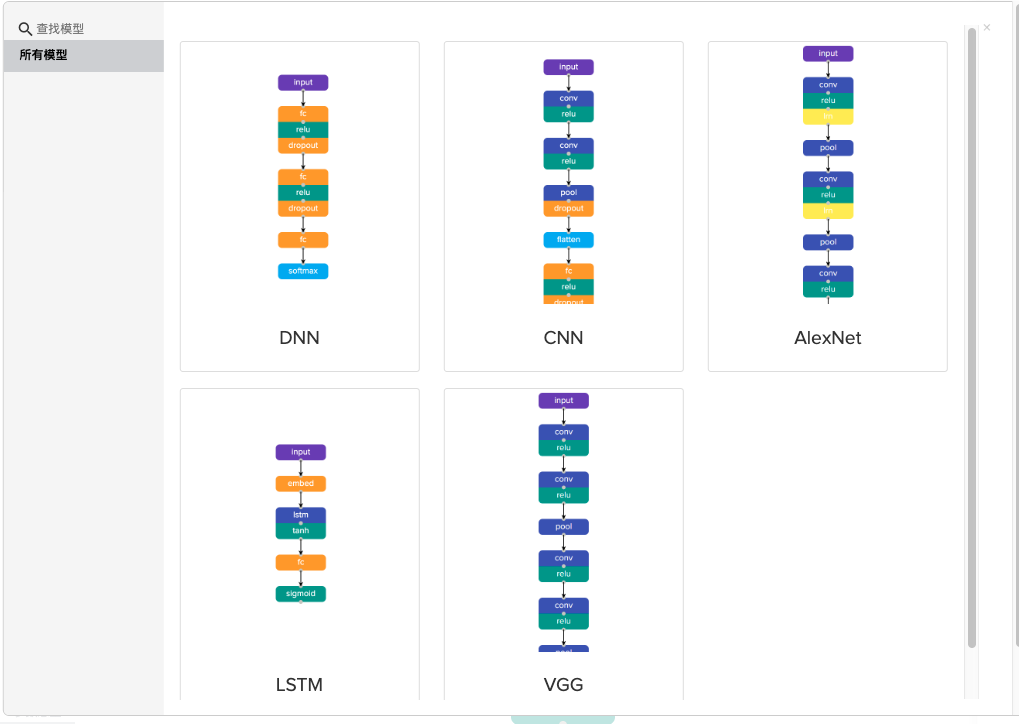
\includegraphics[width=0.98\linewidth]{model.png}
\end{figure}


\section{DNN}





\begin{wrapfigure}{r}{5cm}
\vspace{-1.3cm}

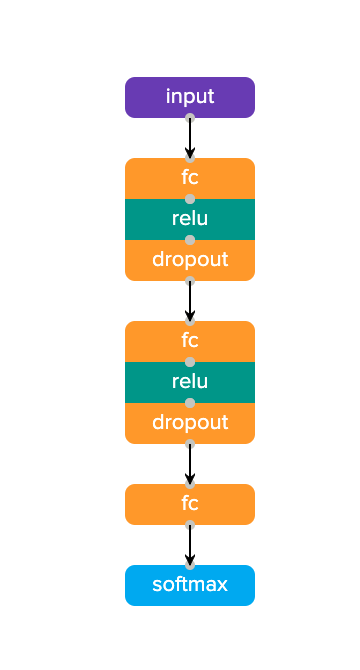
\includegraphics[scale = 0.5]{simple_dnn.png}

\end{wrapfigure}


DNN(Deep Neural Network)神经网络模型又叫全连接神经网络,是基本的深度学习框架。 模型中给出了包含两个隐藏层的深度神经网络,其可以适用于大部分分类(Classification)任务,比如数字识别等。不同于其需要特征工程的机器学习的传统方法(例如高斯混合模型,朴素贝叶斯等),DNN基于原始特征进行端到端学习,相对于传统的机器学习方法有着更好的鲁棒性。

 深度神经网络DNN是基于感知机的扩展,而DNN可以理解为有很多隐藏层的神经网络。DNN有时也叫做多层感知机(Multi-Layer perceptron,MLP)。从DNN按不同层的位置划分,DNN内部的神经网络层可以分为三类,输入层,隐藏层和输出层,如下图示例,一般来说第一层是输出层,最后一层是输出层,而中间的层数都是隐藏层。


 DNN网络中层与层之间是全连接的,也就是说,第i层的任意一个神经元一定与第i+1层的任意一个神经元相连。虽然DNN看起来很复杂,但是从小的局部模型来说,还是和感知机一样,即一个线性关系$\sum{w_ix_i}+b$加上一个激活函数$\sigma(z)$。因此DNN是一种具备至少一个隐藏层的,利用激活函数去线性化,使用交叉熵作损失函数,利用反向传播优化算法(随机梯度下降算法、批量梯度下降算法)进行学习训练(调整并更新神经元之间的权重)的前馈神经网络。
 
 
 \begin{figure}[H]
  \centering
  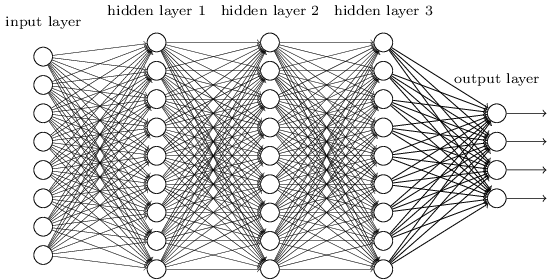
\includegraphics[scale = 0.5]{dnn_show.png}
\end{figure}


\section{CNN}




 卷积神经网络(Convolutional Neural Networks, CNN)是一类包含卷积计算且具有深度结构的前馈神经网络(Feedforward Neural Networks),是深度学习(deep learning)的代表算法之一.卷积神经网络长期以来被大量应用于计算机视觉、自然语言处理等方面,是图像识别领域的核心算法之一,并在大量学习数据时有稳定的表现,还可以用于物体识别、行为认知、遥感科学与大气科学诸多领域。
\begin{wrapfigure}{r}{5cm}


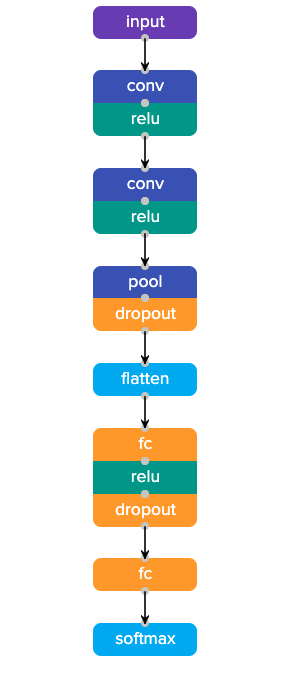
\includegraphics[scale = 0.5]{cnn.png}

\end{wrapfigure}




卷积神经网络是近年发展起来的,并引起广泛重视的一种高效识别方法,20世纪60年代,Hubel和Wiesel在研究猫脑皮层中用于局部敏感和方向选择的神经元时发现其独特的网络结构可以有效地降低反馈神经网络的复杂性,继而提出了卷积神经网络(Convolutional Neural Networks-简称CNN)。现在,CNN已经成为众多科学领域的研究热点之一,特别是在模式分类领域,由于该网络避免了对图像的复杂前期预处理,可以直接输入原始图像,因而得到了更为广泛的应用。 K.Fukushima在1980年提出的新识别机是卷积神经网络的第一个实现网络。随后,更多的科研工作者对该网络进行了改进。其中,具有代表性的研究成果是Alexander和Taylor提出的“改进认知机”,该方法综合了各种改进方法的优点并避免了耗时的误差反向传播。

  这听起来像是一个奇怪的生物学和数学的结合,但是这些网络已经成为计算机视觉领域最具影响力的创新之一。2012年是神经网络成长的第一年,Alex Krizhevsky用它们赢得了当年的ImageNet竞赛(基本上是计算机视觉年度奥运会),把分类错误记录从26%降到了15%,这个惊人的提高从那以后,许多公司一直在以服务为核心进行深度学习。Facebook使用自动标记算法的神经网络,谷歌的照片搜索,亚马逊的产品推荐,Pinterest的家庭饲料个性化和Instagram的搜索基础设施。

\begin{figure}[H]
  \centering
  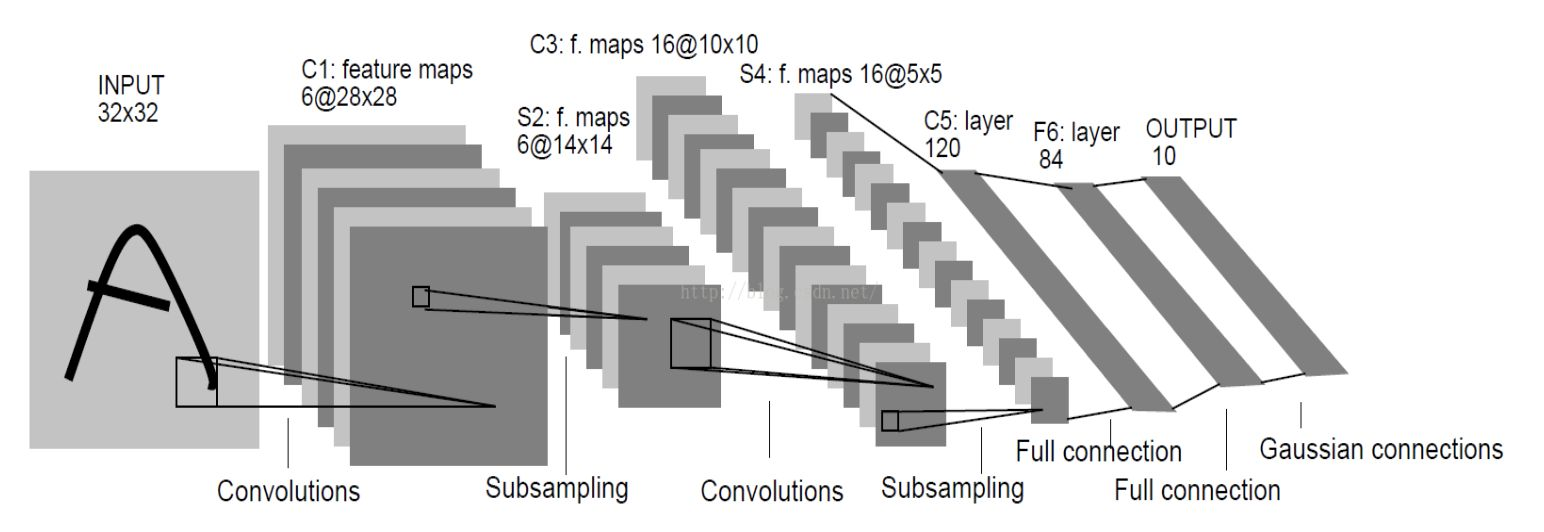
\includegraphics[scale = 0.6]{cnn_show.jpeg}
\end{figure}

一般的,CNN的基本结构包括两层,其一为特征提取层,每个神经元的输入与前一层的局部接受域相连,并提取该局部的特征。一旦该局部特征被提取后,它与其它特征间的位置关系也随之确定下来;其二是特征映射层,网络的每个计算层由多个特征映射组成,每个特征映射是一个平面,平面上所有神经元的权值相等。特征映射结构采用影响函数核小的sigmoid函数作为卷积网络的激活函数,使得特征映射具有位移不变性。此外,由于一个映射面上的神经元共享权值,因而减少了网络自由参数的个数。卷积神经网络中的每一个卷积层都紧跟着一个用来求局部平均与二次提取的计算层,这种特有的两次特征提取结构减小了特征分辨率。

CNN一个非常重要的特点就是头重脚轻(越往输入权值越小,越往输出权值越多),呈现出一个倒三角的形态,这就很好地避免了BP神经网络中反向传播的时候梯度损失得太快。由于CNN的特征检测层通过训练数据进行学习,所以在使用CNN时,避免了显式的特征抽取,而隐式地从训练数据中进行学习;再者由于同一特征映射面上的神经元权值相同,所以网络可以并行学习,这也是卷积网络相对于神经元彼此相连网络的一大优势。卷积神经网络以其局部权值共享的特殊结构在语音识别和图像处理方面有着独特的优越性,其布局更接近于实际的生物神经网络,权值共享降低了网络的复杂性,特别是多维输入向量的图像可以直接输入网络这一特点避免了特征提取和分类过程中数据重建的复杂度。


\section{LSTM}

\begin{wrapfigure}{r}{5cm}

\vspace{-0.9cm}
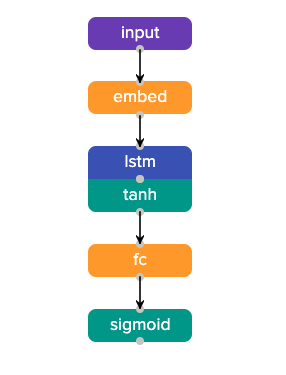
\includegraphics[scale = 0.5]{lstm.png}

\end{wrapfigure}
LSTM(Long Short-Term Memory)是长短期记忆网络,是一种时间循环神经网络,适合于处理和预测时间序列中间隔和延迟相对较长的重要事件。 LSTM 已经在科技领域有了多种应用。基于 LSTM 的系统可以学习翻译语言、控制机器人、图像分析、文档摘要、语音识别图像识别、手写识别、控制聊天机器人、预测疾病、点击率和股票、合成音乐等等任务。

LSTM是为了避免长依赖问题而精心设计的。 记住较长的历史信息实际上是他们的默认行为,而不是他们努力学习的东西。所有循环神经网络都具有神经网络的重复模块链的形式。 在标准的RNN中,该重复模块将具有非常简单的结构,例如单个tanh层。LSTM也拥有这种链状结构,但是重复模块则拥有不同的结构。与神经网络的简单的一层相比,LSTM拥有四层,这四层以特殊的方式进行交互。
\begin{figure}[H]
  \centering
  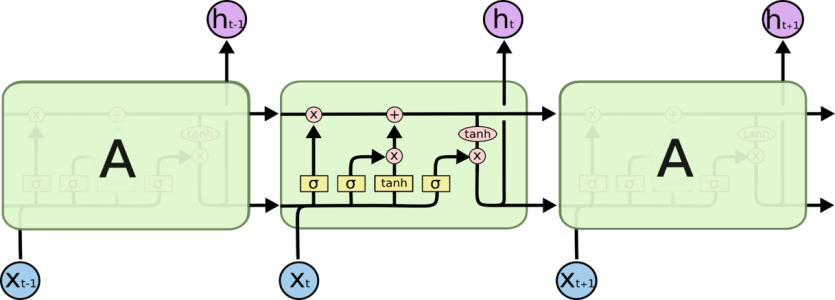
\includegraphics[scale = 0.4]{lstm_show.jpg}
\end{figure}

首先,在新数据传入LSTM时,我们要决定哪些旧数据需要从cell state中扔掉。这个就是由forget gate决定的,它是一个sigmoid函数层。

​第二步是决定哪些新的信息需要被存储进cell state,分为两个步骤。首先,一个sigmoid函数层,即inpu gate会决定哪些值需要被更新;然后,一个tanh函数层会创建一个向量,作为加入到cell state的候选值。

​之后就可以更新cell state,这同样分为两步。首先,我们从cell state移除掉我们在forget gate决定的信息;然后,我们以决定对每一个状态值更新的比例来加入input gate计算出的候选值。

最后,我们决定将要输出的部分。输出是基于新的cell state,同时进行适当的处理。首先,我们通过一个sigmoid函数层来决定cell state中有哪些部分需要被更新,然后,我们将cell state经过一个tanh函数处理(其目的是使得数值落在(-1,1)区间内),并将其余sigmoid层的输出相乘,从而决定输出的部分。

​对于绝大部分问题,LSTM 相比于RNN更好用,LSTM 是 RNN 取得的一大进步。然而LSTM还有其他的进步空间,那就是注意力(attention)。注意力的想法是让 RNN 中的每一步都从信息更加富集的地方提取信息。例如,你想使用 RNN 对一幅图片生成描述,它也需要提取图片中的一部分来生成输出的文字。注意力并非 RNN 研究中唯一一个激动人心的思路。Kalchbrenner 等人提出的 Grid LSTM 看起来极具潜力。Gregor等人、Chung 等人,或者 Bayer 与 Osendorfer 在生成模型中使用 RNN 的想法也非常有意思。最近几年是递归神经网络的风口时期,新出的成果只会更具前景。

\section{AlexNet}

\begin{wrapfigure}{r}{5cm}


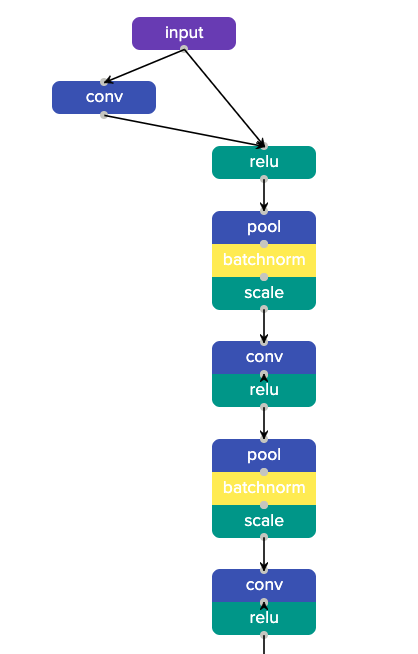
\includegraphics[scale = 0.5]{alexnet.png}

\end{wrapfigure}

虽然CNN在图像分类中取得了较好的成绩,但是由于计算机性能的影响,并没有广泛使用。 直到2012年,Alex等人提出的**AlexNet**网络在ImageNet大赛上以远超第二名的成绩夺冠, 将错误率降低至16.4\% ,卷积神经网络乃至深度学习重新引起了关注。AlexNet使用Relu函数作为CNN的激活函数,解决了Sigmoid在深层网络的梯度弥散问题。提出了LRN层,对局部神经元的活动创建竞争机制,使其影响大的值变化相对大,抑制反馈较小的神经元,增强了模型泛化能力。

Alexnet是由5个卷积层和三个全连接层组成,一共8个权重层(池化层不是权重层因为其没有参数),其中ReLU激活函数作用在每个卷积层和全连接层上,在第一个卷积层和第二个卷积层后面连接一个局部响应规范化层,最大池化层作用在第一个卷积层,第二个卷积层和第五个卷积层的输出上。

​通常在卷积层后面都应该接一个池化层,但是AlexNet却只在第一个卷积层,第二个卷积层和最后一个卷积层后面连接最大池化,这是因为在网络的较低层,特征映射的大小一般很大,含有较多的参数,这是进行池化的目的是为了减少的参数的数量,防止过拟合,而在网络的较高层,提取的特征一般是高级特征,可能是某个物体的轮廓,比如小狗的眼睛,但是小狗可能出现在图像中的任意位置,此时最大池化的目的是提供一种平移翻转不变性。至于AlexNet为什么只用了5个卷积层,论文中提到深度是重要的,但是再深可能会出现退化现象。而去掉一个卷积层又会使网络的表示能力下降。

\begin{figure}[H]
  \centering
  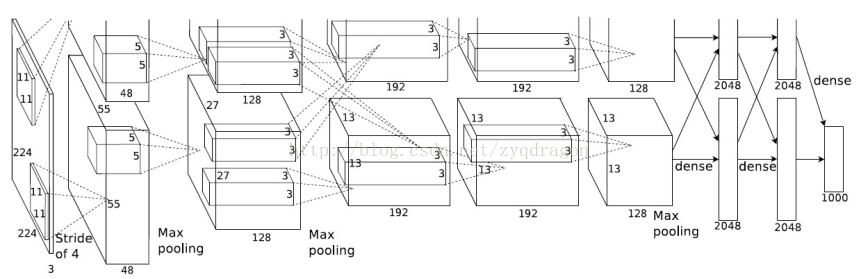
\includegraphics[scale = 0.6]{alexnet_show.png}
\end{figure}

就梯度下降训练时间而言,饱和非线性函数:sigmoid函数或tanh函数比非饱和非线性函数:ReLU函数用时长。AlexNet网络的激活函数使用ReLU函数,加快了神经网络的训练速度。现在ReLU函数几乎成为深度网络默认使用的激活函数。使用数据增强策略和随机失活策略(dropout) 防止训练数据过拟合,至今被很多网络借鉴。AlexNet网络采用连续卷积结合汇合层,最后是全连接层的方式,仍然是现今最先进网络的基础。

​因此AlexNet网络有两点重要的意义,首先是AlexNet网络使用的诸多项设置成为卷积神经网络常见的默认设置,仍被广泛应用。此外,它也使研究者们意识到GPU高度优化的2维卷积功能足够支持大型高分辨率数据集上大型CNN网络的训练。


\section{VGG}

\begin{wrapfigure}{r}{5cm}

\vspace{-0.9cm}
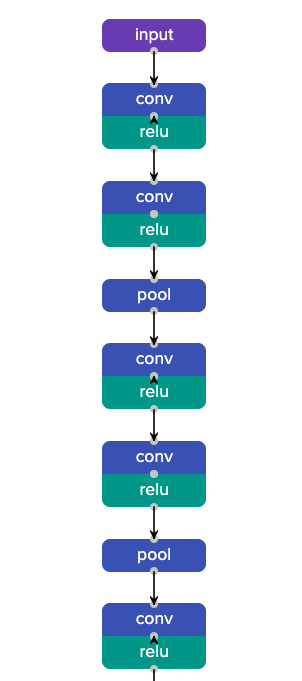
\includegraphics[scale = 0.5]{vgg.png}

\end{wrapfigure}
VGGNet由牛津大学计算机视觉组合和Google DeepMind公司研究员一起研发的深度卷积神经网络。它探索了卷积神经网络的深度和其性能之间的关系,通过反复的堆叠3*3的小型卷积核和2*2的最大池化层,成功的构建了16~19层深的卷积神经网络。VGGNet获得了ILSVRC 2014年比赛的亚军和定位项目的冠军,在top5上的错误率为7.5\%。目前为止,VGGNet依然被用来提取图像的特征。VGGNet可以看成是加深版本的AlexNet,都是由卷积层、全连接层两大部分构成。

相比于之前的神经网络结构,VGG主要有以下的特点:



(1) 结构简洁。VGG由5层卷积层、3层全连接层、softmax输出层构成,层与层之间使用max-pooling(最大化池)分开,所有隐层的激活单元都采用ReLU函数。

(2) 小卷积核和多卷积子层。VGG使用多个较小卷积核(3x3)的卷积层代替一个卷积核较大的卷积层,一方面可以减少参数,另一方面相当于进行了更多的非线性映射,可以增加网络的拟合/表达能力。小卷积核是VGG的一个重要特点,虽然VGG是在模仿AlexNet的网络结构,但没有采用AlexNet中比较大的卷积核尺寸(如7x7),而是通过降低卷积核的大小(3x3),增加卷积子层数来达到同样的性能(VGG:从1到4卷积子层,AlexNet:1子层)。VGG的作者认为两个3x3的卷积堆叠获得的感受野大小,相当一个5x5的卷积;而3个3x3卷积的堆叠获取到的感受野相当于一个7x7的卷积。这样可以增加非线性映射,也能很好地减少参数(例如7x7的参数为49个,而3个3x3的参数为27)。

(3) 小池化核。相比AlexNet的3x3的池化核,VGG全部采用2x2的池化核。

(4) 通道数多。VGG网络第一层的通道数为64,后面每层都进行了翻倍,最多到512个通道,通道数的增加,使得更多的信息可以被提取出来。

(5) 层数更深、特征图更宽。由于卷积核专注于扩大通道数、池化专注于缩小宽和高,使得模型架构上更深更宽的同时,控制了计算量的增加规模。

(6) 全连接转卷积。这也是VGG的一个特点,在网络测试阶段将训练阶段的三个全连接替换为三个卷积,使得测试得到的全卷积网络因为没有全连接的限制,因而可以接收任意宽或高为的输入,这在测试阶段很重要。	



\begin{figure}[H]
  \centering
  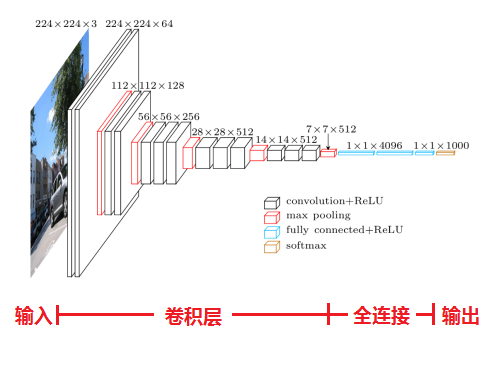
\includegraphics[scale = 0.7]{vgg_show.png}
\end{figure}

VGG模型是2014年ILSVRC竞赛的第二名,第一名是GoogLeNet。但是VGG模型在多个迁移学习任务中的表现要优于googLeNet。而且,从图像中提取CNN特征,VGG模型是首选算法。它的缺点在于,参数量有140M之多,需要更大的存储空间。但是这个模型很有研究价值。


\part{使用说明}


\chapter{mnist用例}

这篇文档里为大家提供一个通过VisualNN来构建一个简单的DNN来进行手写字符识别。具体的步骤可以表示为

1. VisualNN中构建网络结构

2. 导出模型到本地或者HDFS

3. 运行训练脚本得到训练好的权重文件

4. 运行预测脚本进行字符识别
   
   下面我们分节介绍每个步骤




\section{构建网络结构}

这里我们构建一个最简单的三层DNN的分类网路,首先第一步是构建输入层, 这里的主要目的是指定输入的数据的维度.

首先从左侧点击数据section中的Input块, 这会在右侧的panel中添加输入层,然后点击panel中新生成的输入层,右侧会显示出这一层的参数,我们设置右侧的参数为(1, 784), 输入层就构建完成了。

\begin{figure}[H]
  \centering
  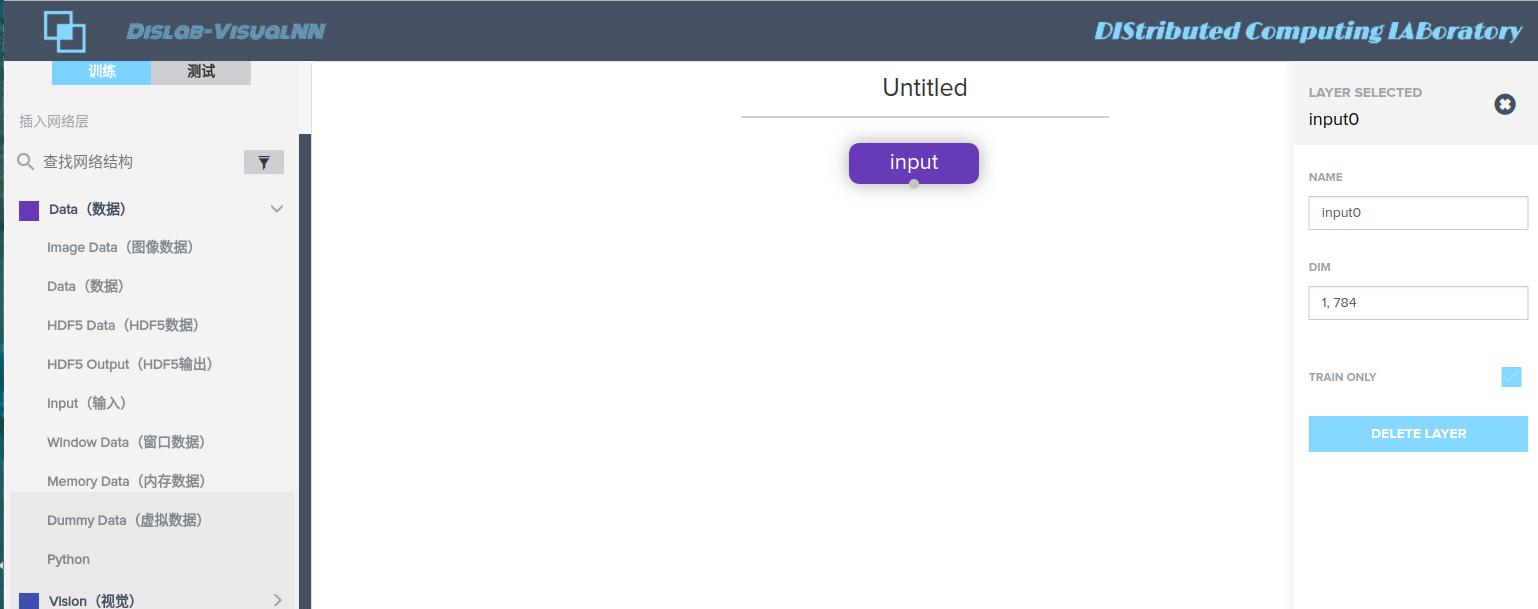
\includegraphics[width=0.98\linewidth]{example_input.png}
\end{figure}


接下来是构建三层的DNN, 我们点击左侧Common中的全连接层,右侧会自动添加一个全连接层并从之前构建的网络中连接一条线到新创建的神经网络层, 如果没有自动连接可以手动连接一下, 之后我在右侧设置全连接层的参数, 可以看到全连接层有很多复杂的参数, 如果不理解请参见tensorflow的文档, 在这里我们设置输出维数为512, 具体过程如下图所示


\begin{figure}[H]
  \centering
  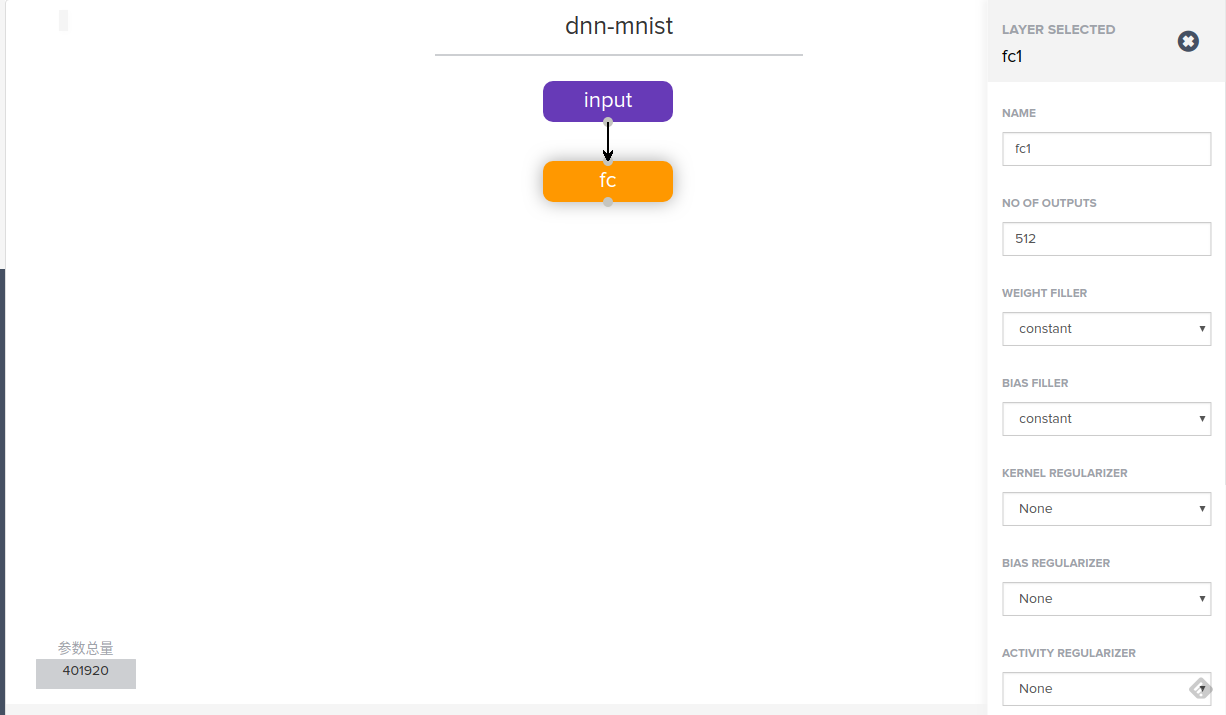
\includegraphics[width=0.98\linewidth]{example_fc.png}
\end{figure}


然后再添加Common中的DropOut层, 我们设置drop的几率为0.2, 如下所示

\begin{figure}[H]
  \centering
  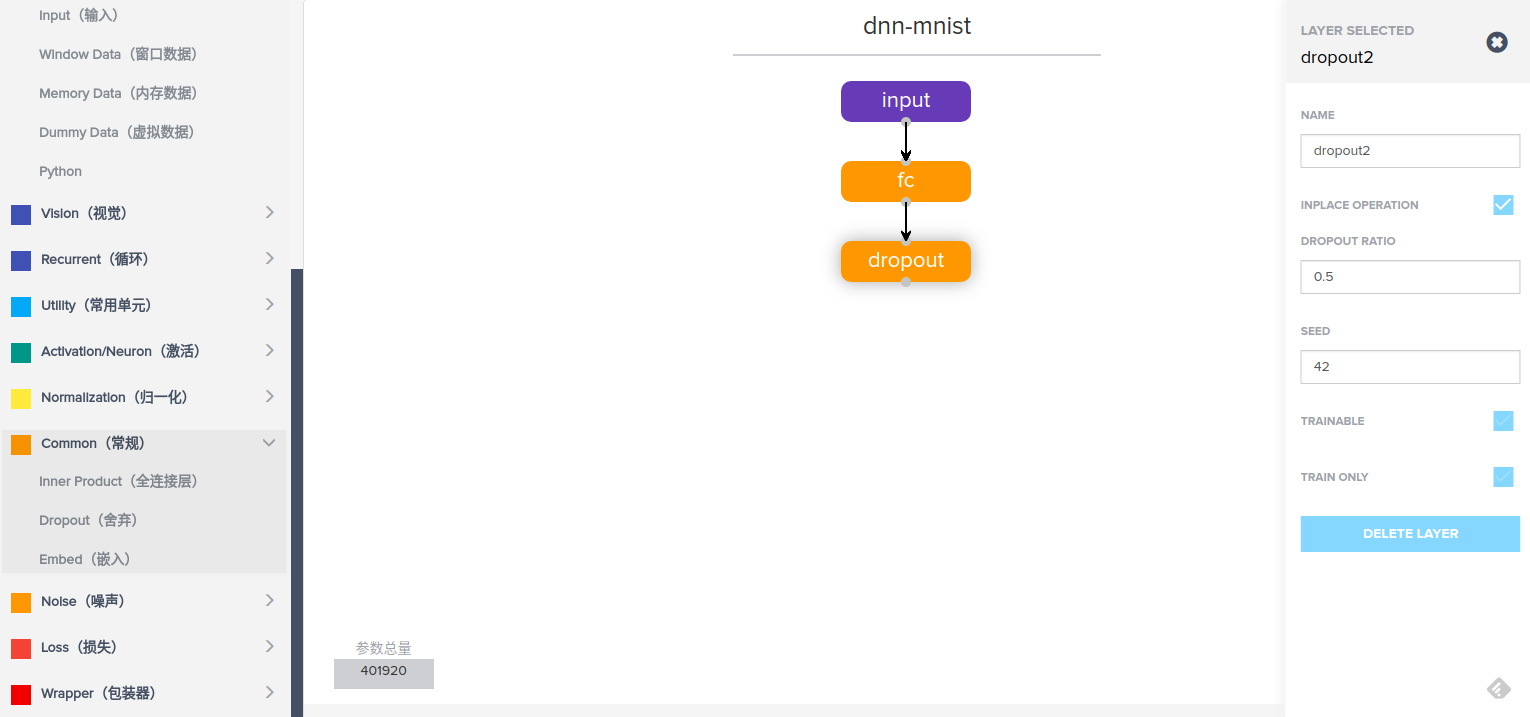
\includegraphics[width=0.98\linewidth]{example_dropout.png}
\end{figure}

然后按照同样的方法在添加两个叠加的DNN和DropOut层, 注意最后一个DNN要将输出维数设置为10, 因为我们要进行手写字符识别(0~9),总共10个数字, 具体如下图所示。

\begin{figure}[H]
  \centering
  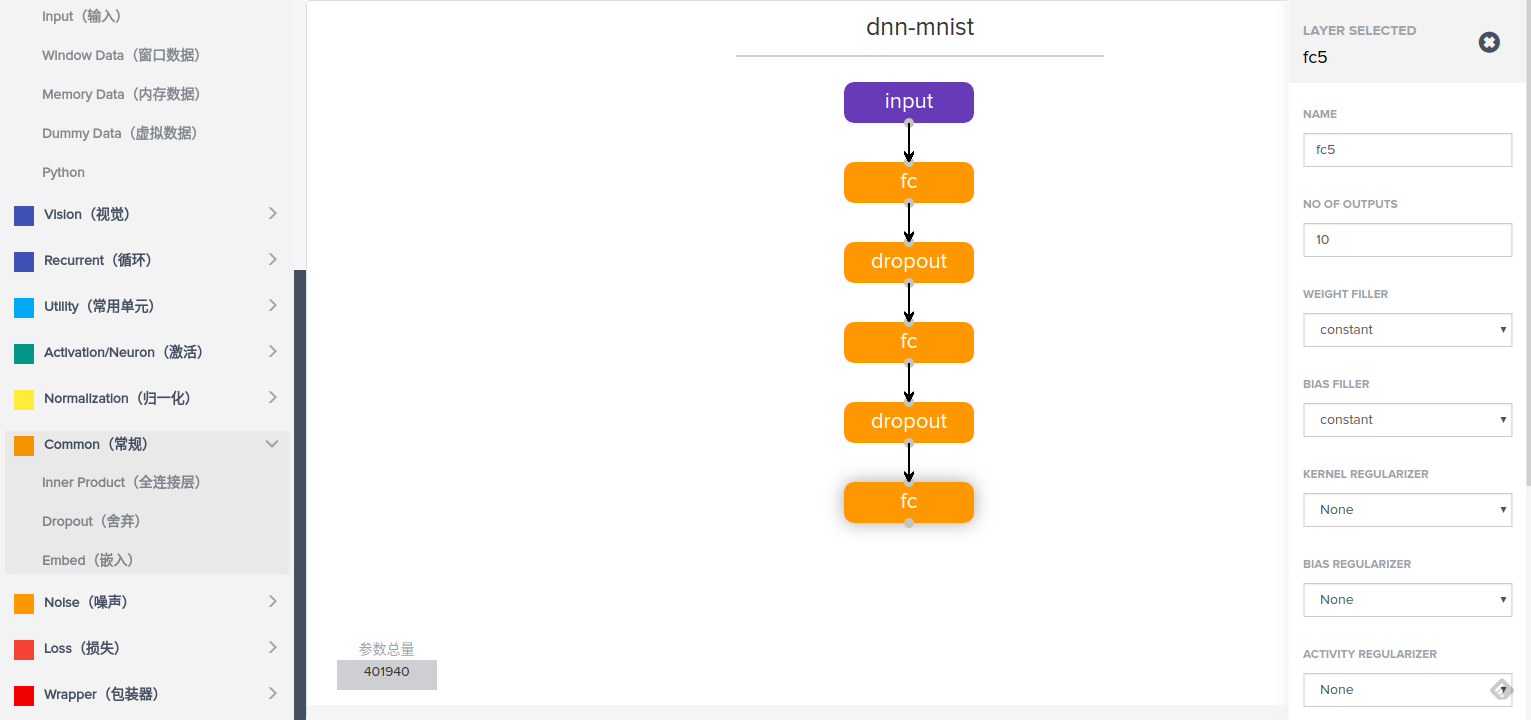
\includegraphics[width=0.98\linewidth]{example_three_dnn.png}
\end{figure}


最后再添加一个Utility中的softmax层, 不需要设置参数,softmax层将会输出每个类别的概率, 如下图所示。

\begin{figure}[H]
  \centering
  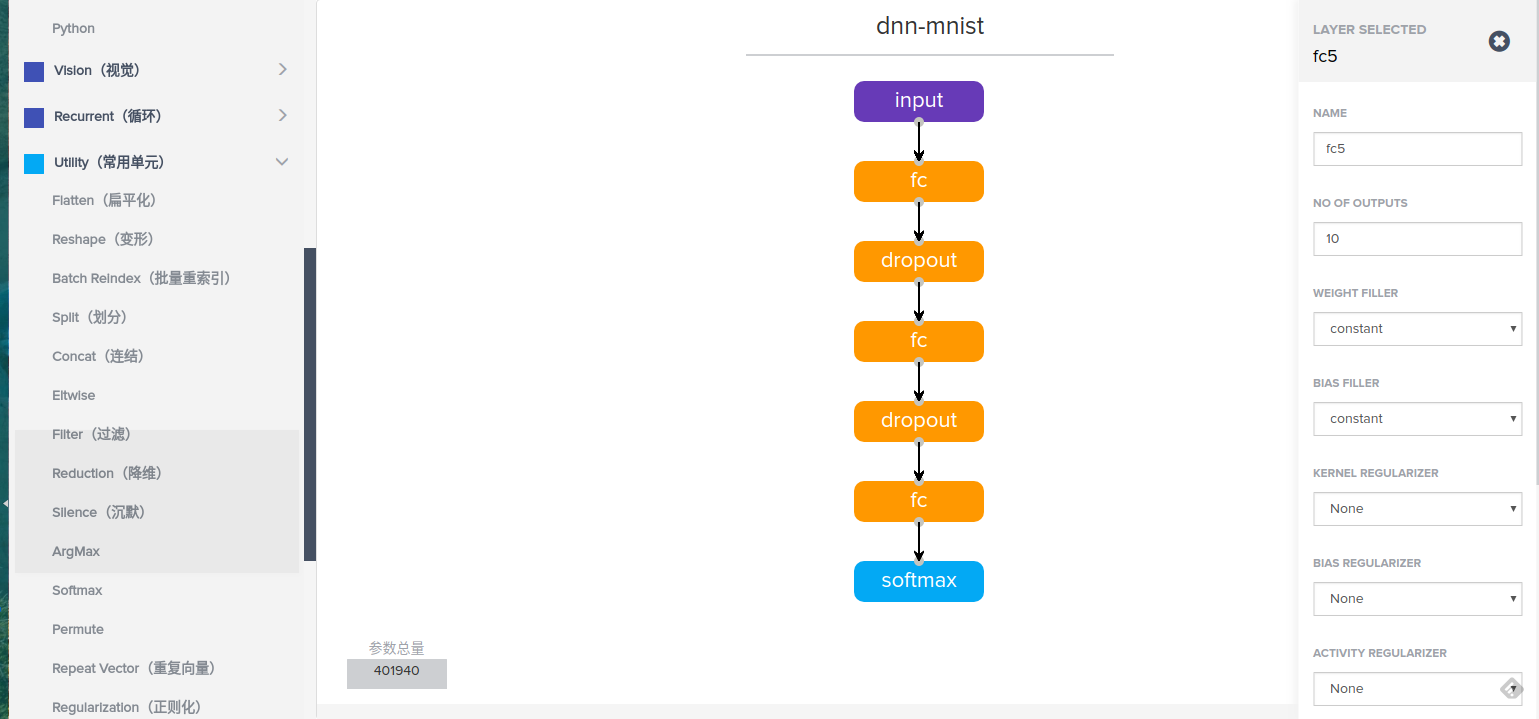
\includegraphics[width=0.98\linewidth]{example_softmax.png}
\end{figure}
至此我们已经构建完成了一个简单的DNN网络, 下一步就是导出模型

\section{导出模型}

点击左侧export功能下的keras可以将模型导出到本地磁盘,或者导出到HDFS上(未完成)TODO, 在导出的同时会在数据库中插入一个算子, 具体导出过程如下图所示
\begin{figure}[H]
  \centering
  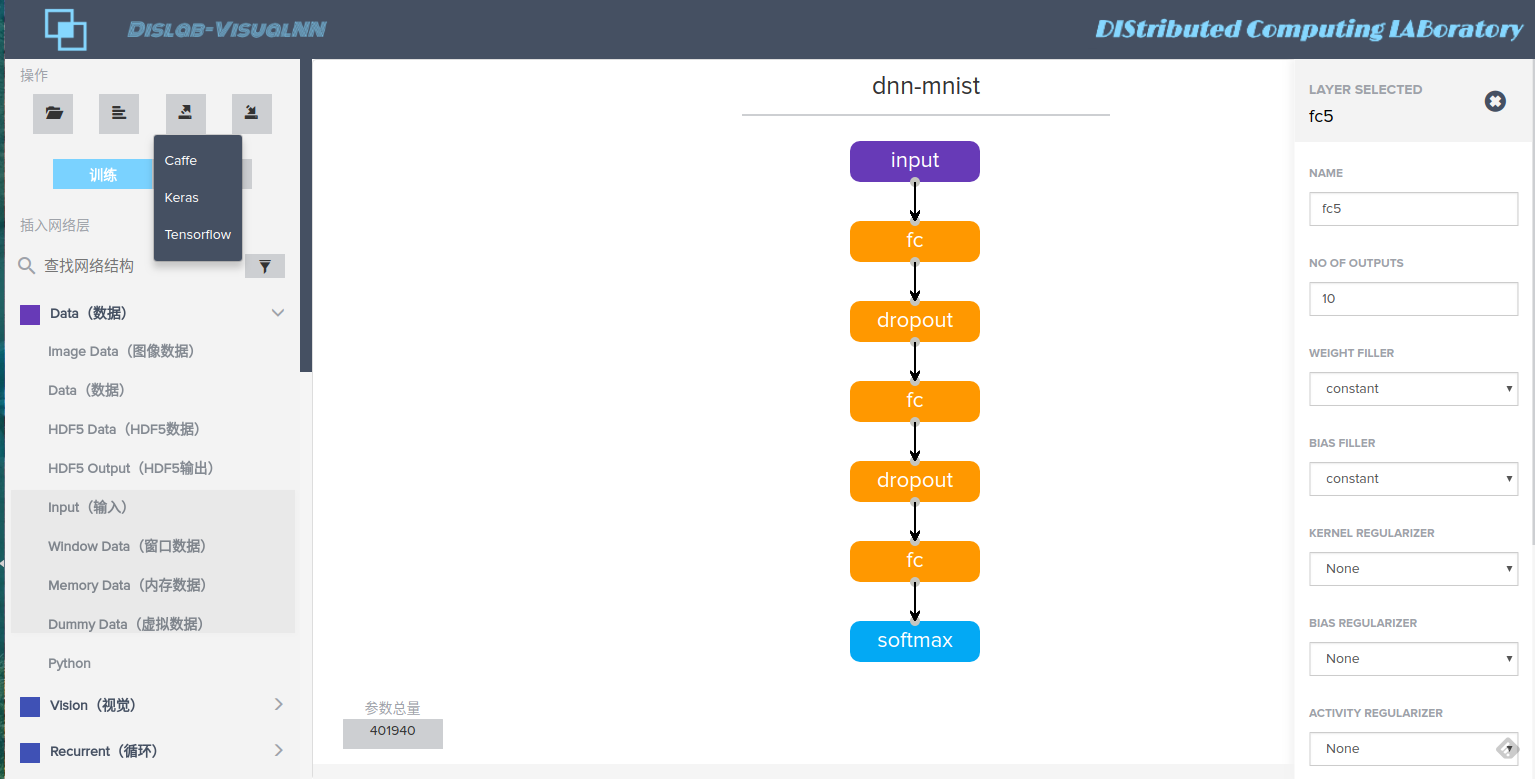
\includegraphics[width=0.98\linewidth]{example_export.png}
\end{figure}

在这次演示中我们将刚刚搭建好的模型导出到本地磁盘上, 比如导出到VisualNN项目目录model下的dnn\_mnist.json。

\section{运行训练脚本}
训练脚本保存在script目录下的train.py文件, 输入参数格式为TODO, 我们可以按照下面的方式调用这个训练脚本

\begin{lstlisting}[%
language=golang,
caption={code sample},
label=lst:golangexample
]
python train.py ../models/temp.json
 ~/.keras/datasets/preprocessing_minist.npz temp.h5
\end{lstlisting}

\begin{figure}[H]
  \centering
  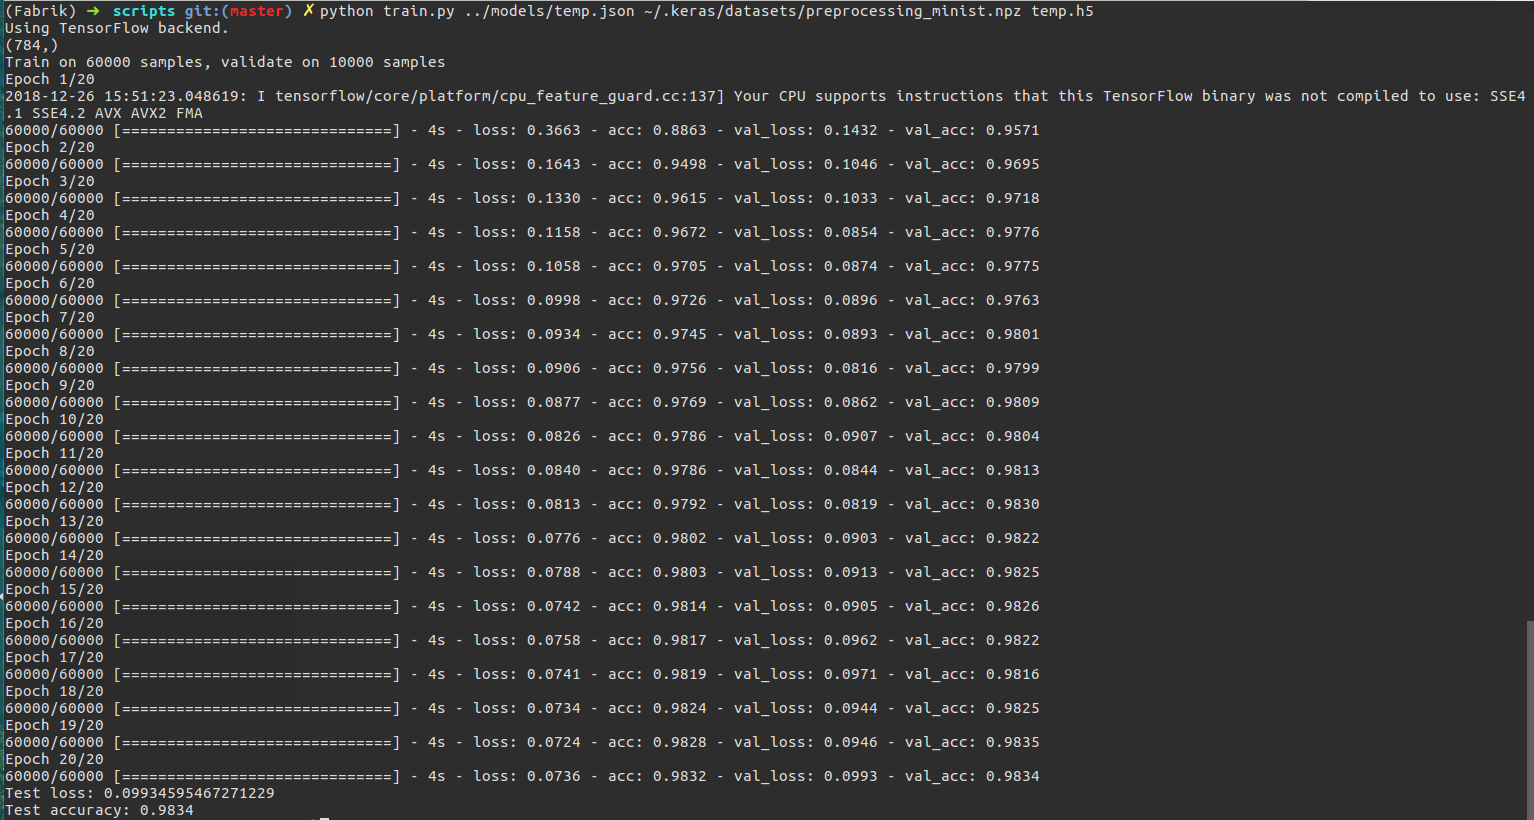
\includegraphics[width=0.98\linewidth]{example_train.png}
\end{figure}

上面参数从左到右分别是模型结构文件, 训练数据集路径, 权重输出路径。训练过程会输出迭代过程中的精度, 如下图所示,训练得到的权重文件将保到指定的目录下。

\begin{figure}[H]
  \centering
  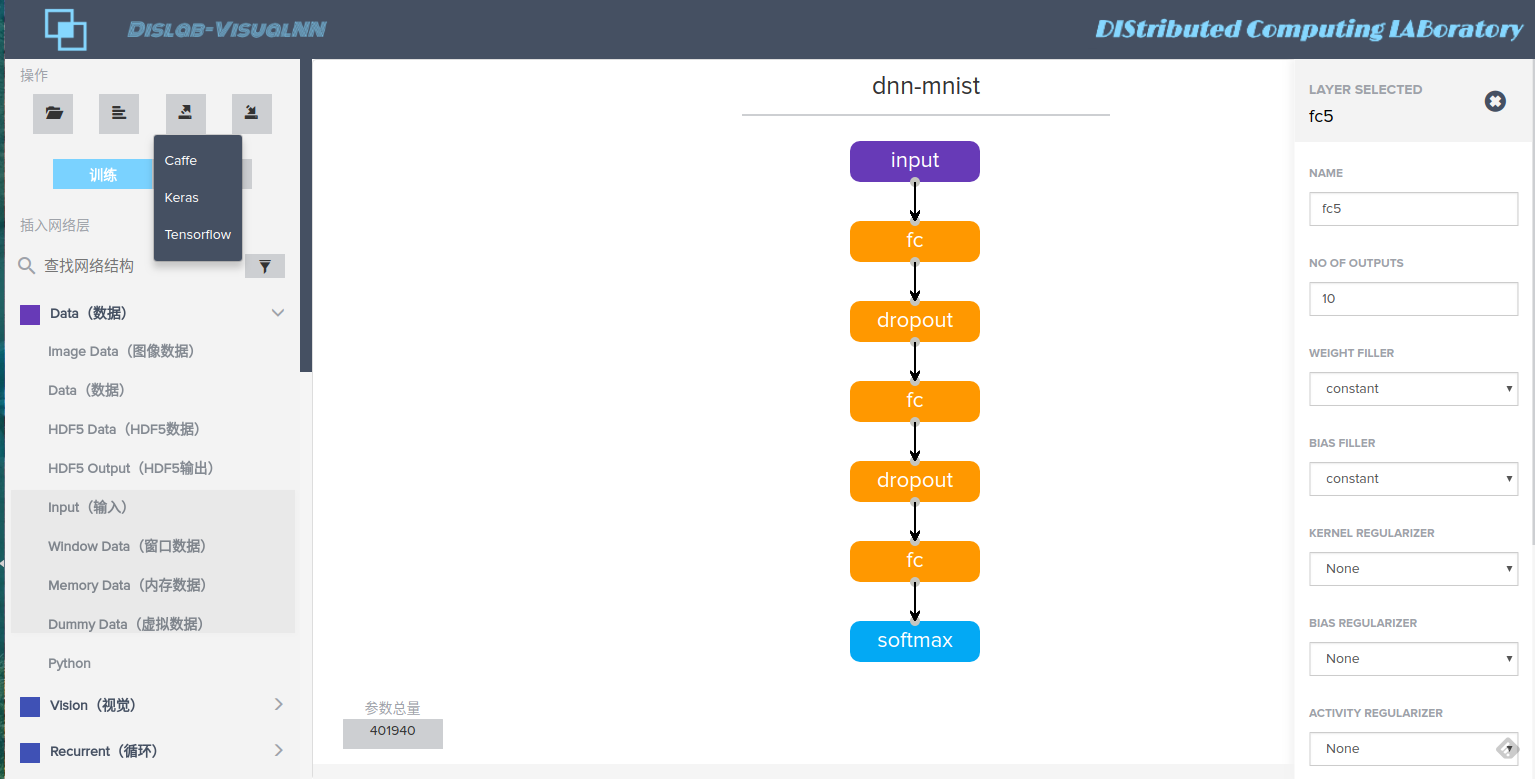
\includegraphics[width=0.98\linewidth]{example_export.png}
\end{figure}

\section{模型测试}

测试脚本保存在script下的eval.py, 具体调用方法如下所示

\begin{lstlisting}[%
language=golang,
caption={code sample},
label=lst:golangexample
]
python eval.py ../models/vgg16.json
../models/vgg16_weights_tf_dim_ordering_tf_kernels.h5 
../models/data/test/Coffee-Mug.jpg
\end{lstlisting}

目前预测结果采用的方式是输出到标准输出,可以通过重定向的方法输出到文件中从而进行后续操作

\bookmarksetup{startatroot}





%% 参考文献
\bibliographystyle{plain}

\end{document}

%%% Local Variables:
%%% mode: latex
%%% TeX-master: t
%%% End:
